\chapter{Resultados}\label{ch:results}
En los siguientes experimentos se trabaja con una epidemia con una tasa de contagio $\beta = 1.5$ y una tasa de recuperación de $\gamma = 1$
\section{Vacunación}
Se sabe que las vacunas son una medida de contingencia efectiva contra una epidemia, lo que se quiere mostrar con este experimento es la diferencia entre la cantidad de infectados cuando se eligen distintas estrategias de vacunación. 

Se trabaja con dos distintas estrategias, una es la vacunación aleatoria y la otra es tomando en cuenta los nodos que más influyen en la red. En ambos experimentos se varía la cantidad de nodos vacunados desde el inicio de la epidemia, es decir, tienen un estado de \textit{recuperado} desde el inicio. 

En la figura \ref{fig:random} tenemos los resultados de utilizar la estrategia aleatoria y en la figura \ref{fig:influential-nodes} los resultados de vacunar influyentes. Como se nota en ambas, la cantidad final de infectados disminuye conforme la cantidad de vacunados crece, pero se nota que la disminución es mayor cuando se vacunan a \textit{personas} influyentes.

\begin{figure}
    \centering
    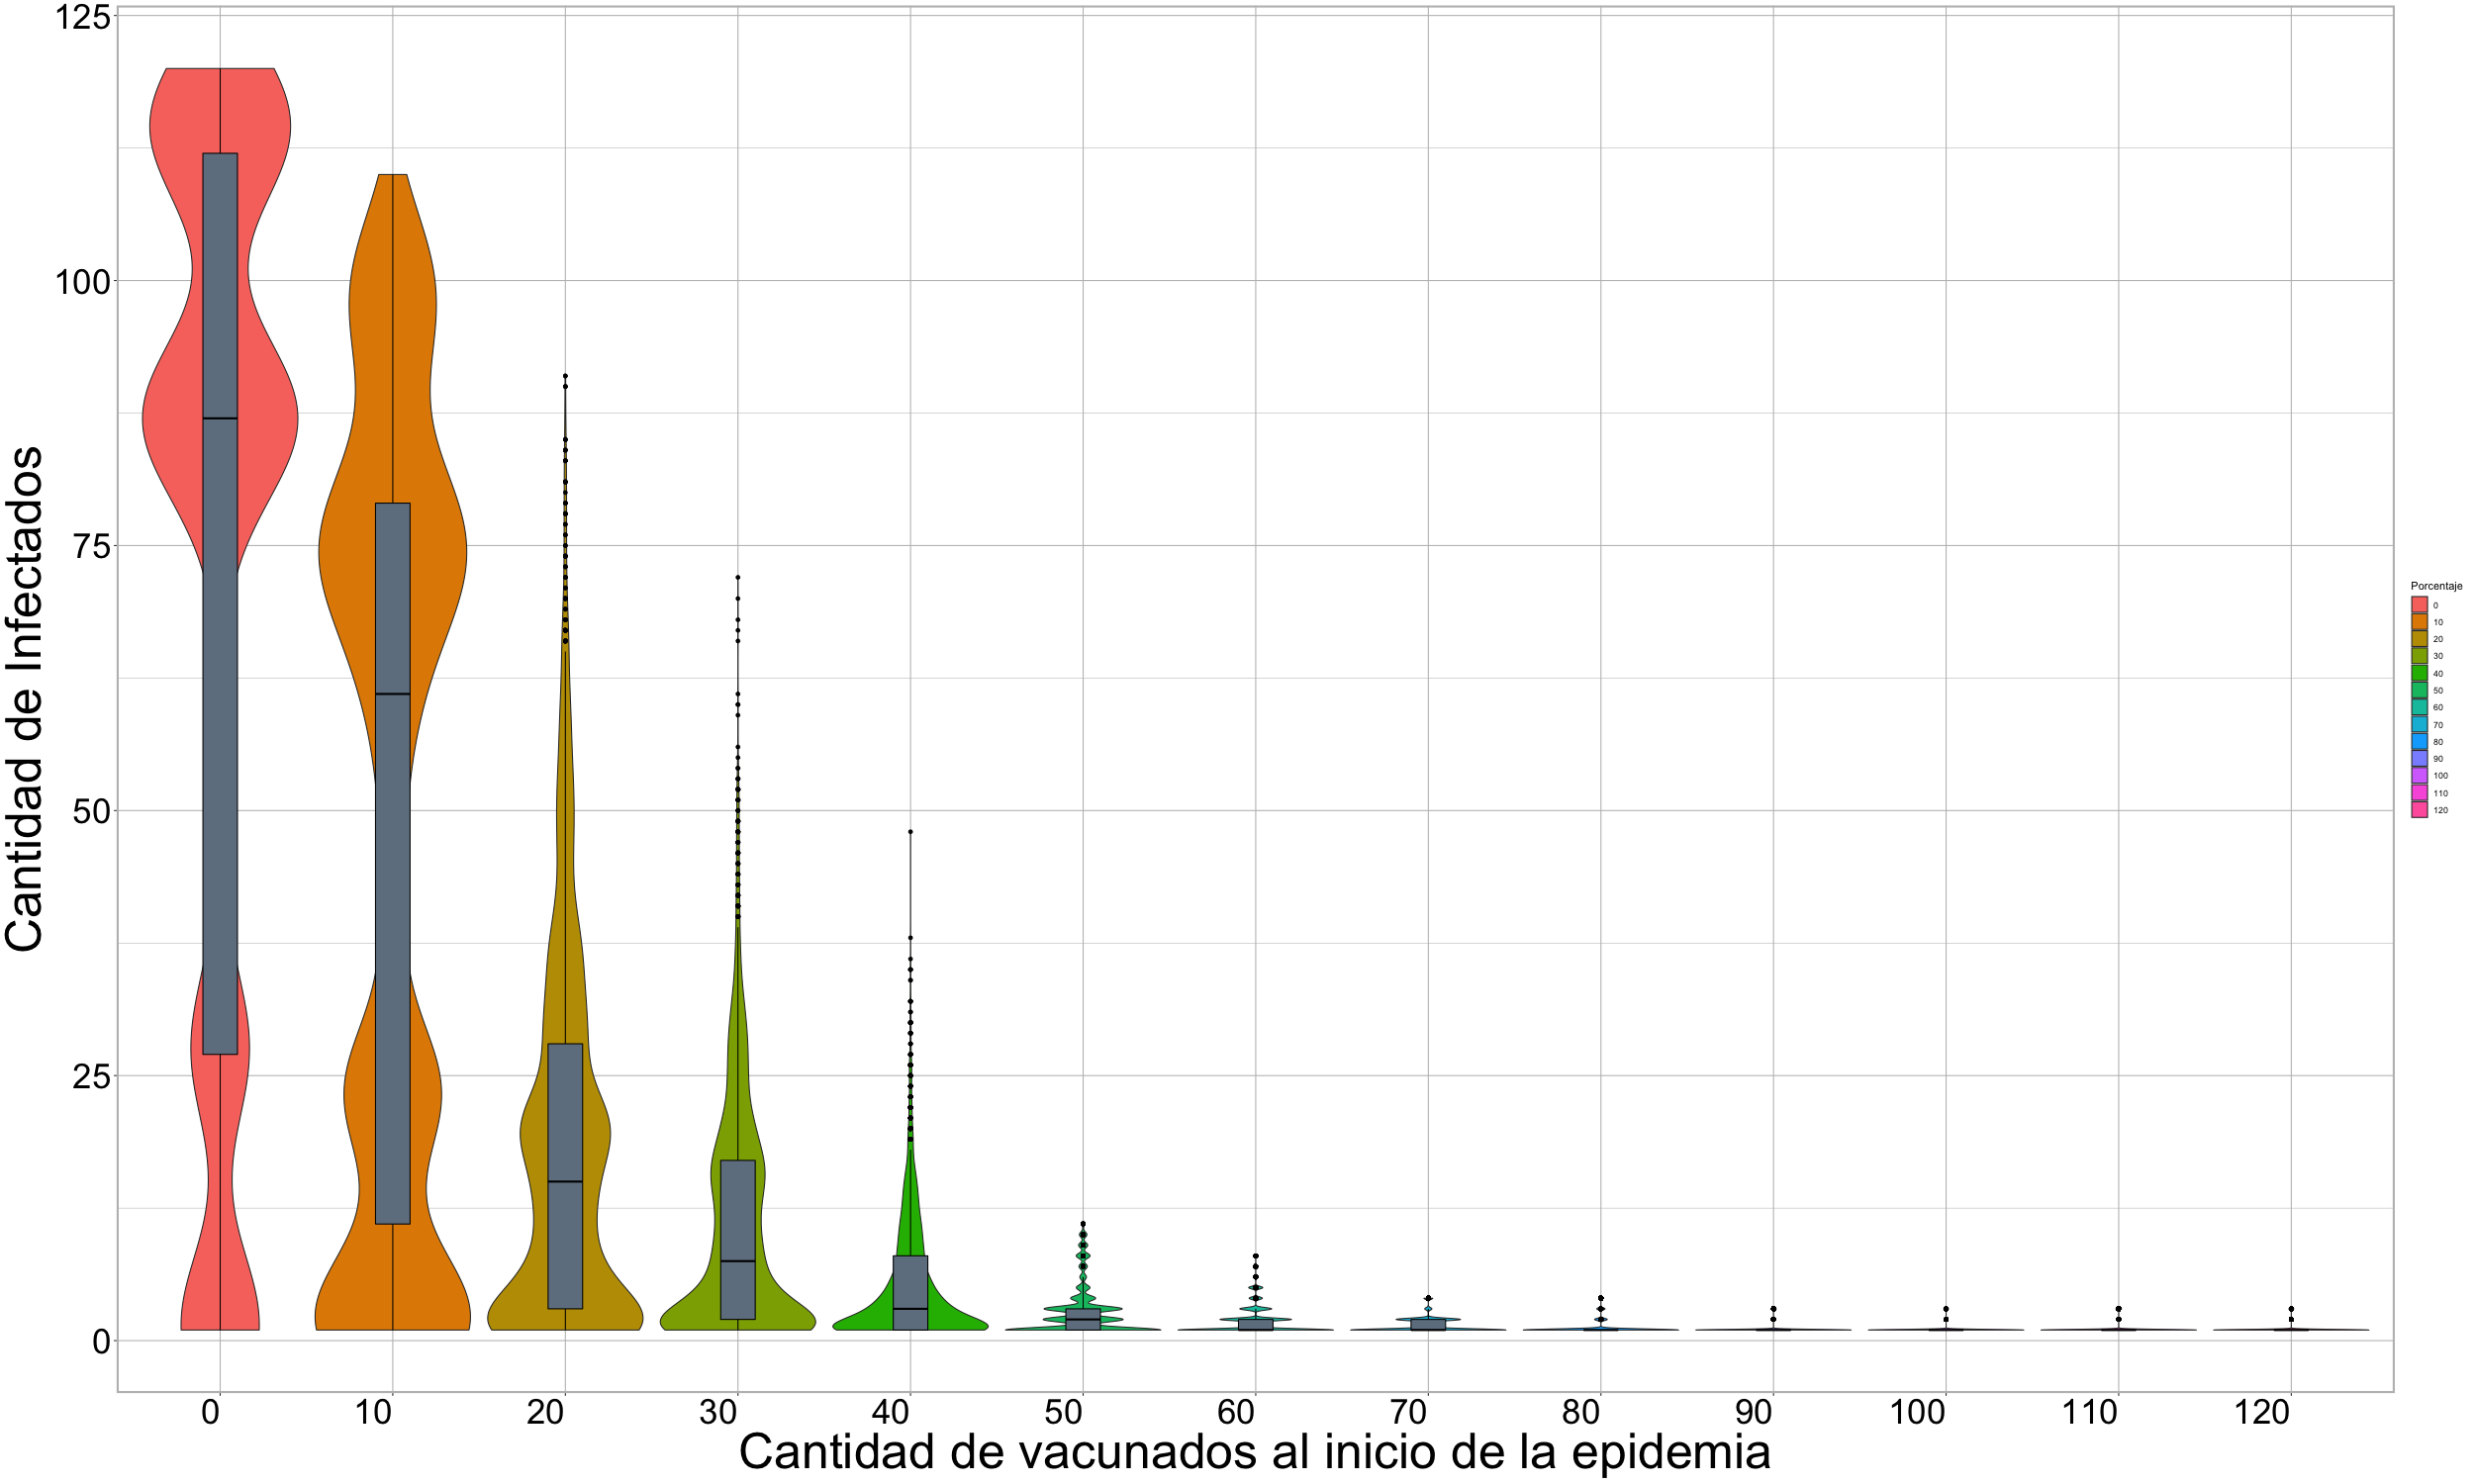
\includegraphics[scale=0.18]{Tesis/img/influential-nodes.png}
    \caption{Vacunando a los nodos influyentes de la red.}
    \label{fig:influential-nodes}
\end{figure}

\begin{figure}
    \centering
    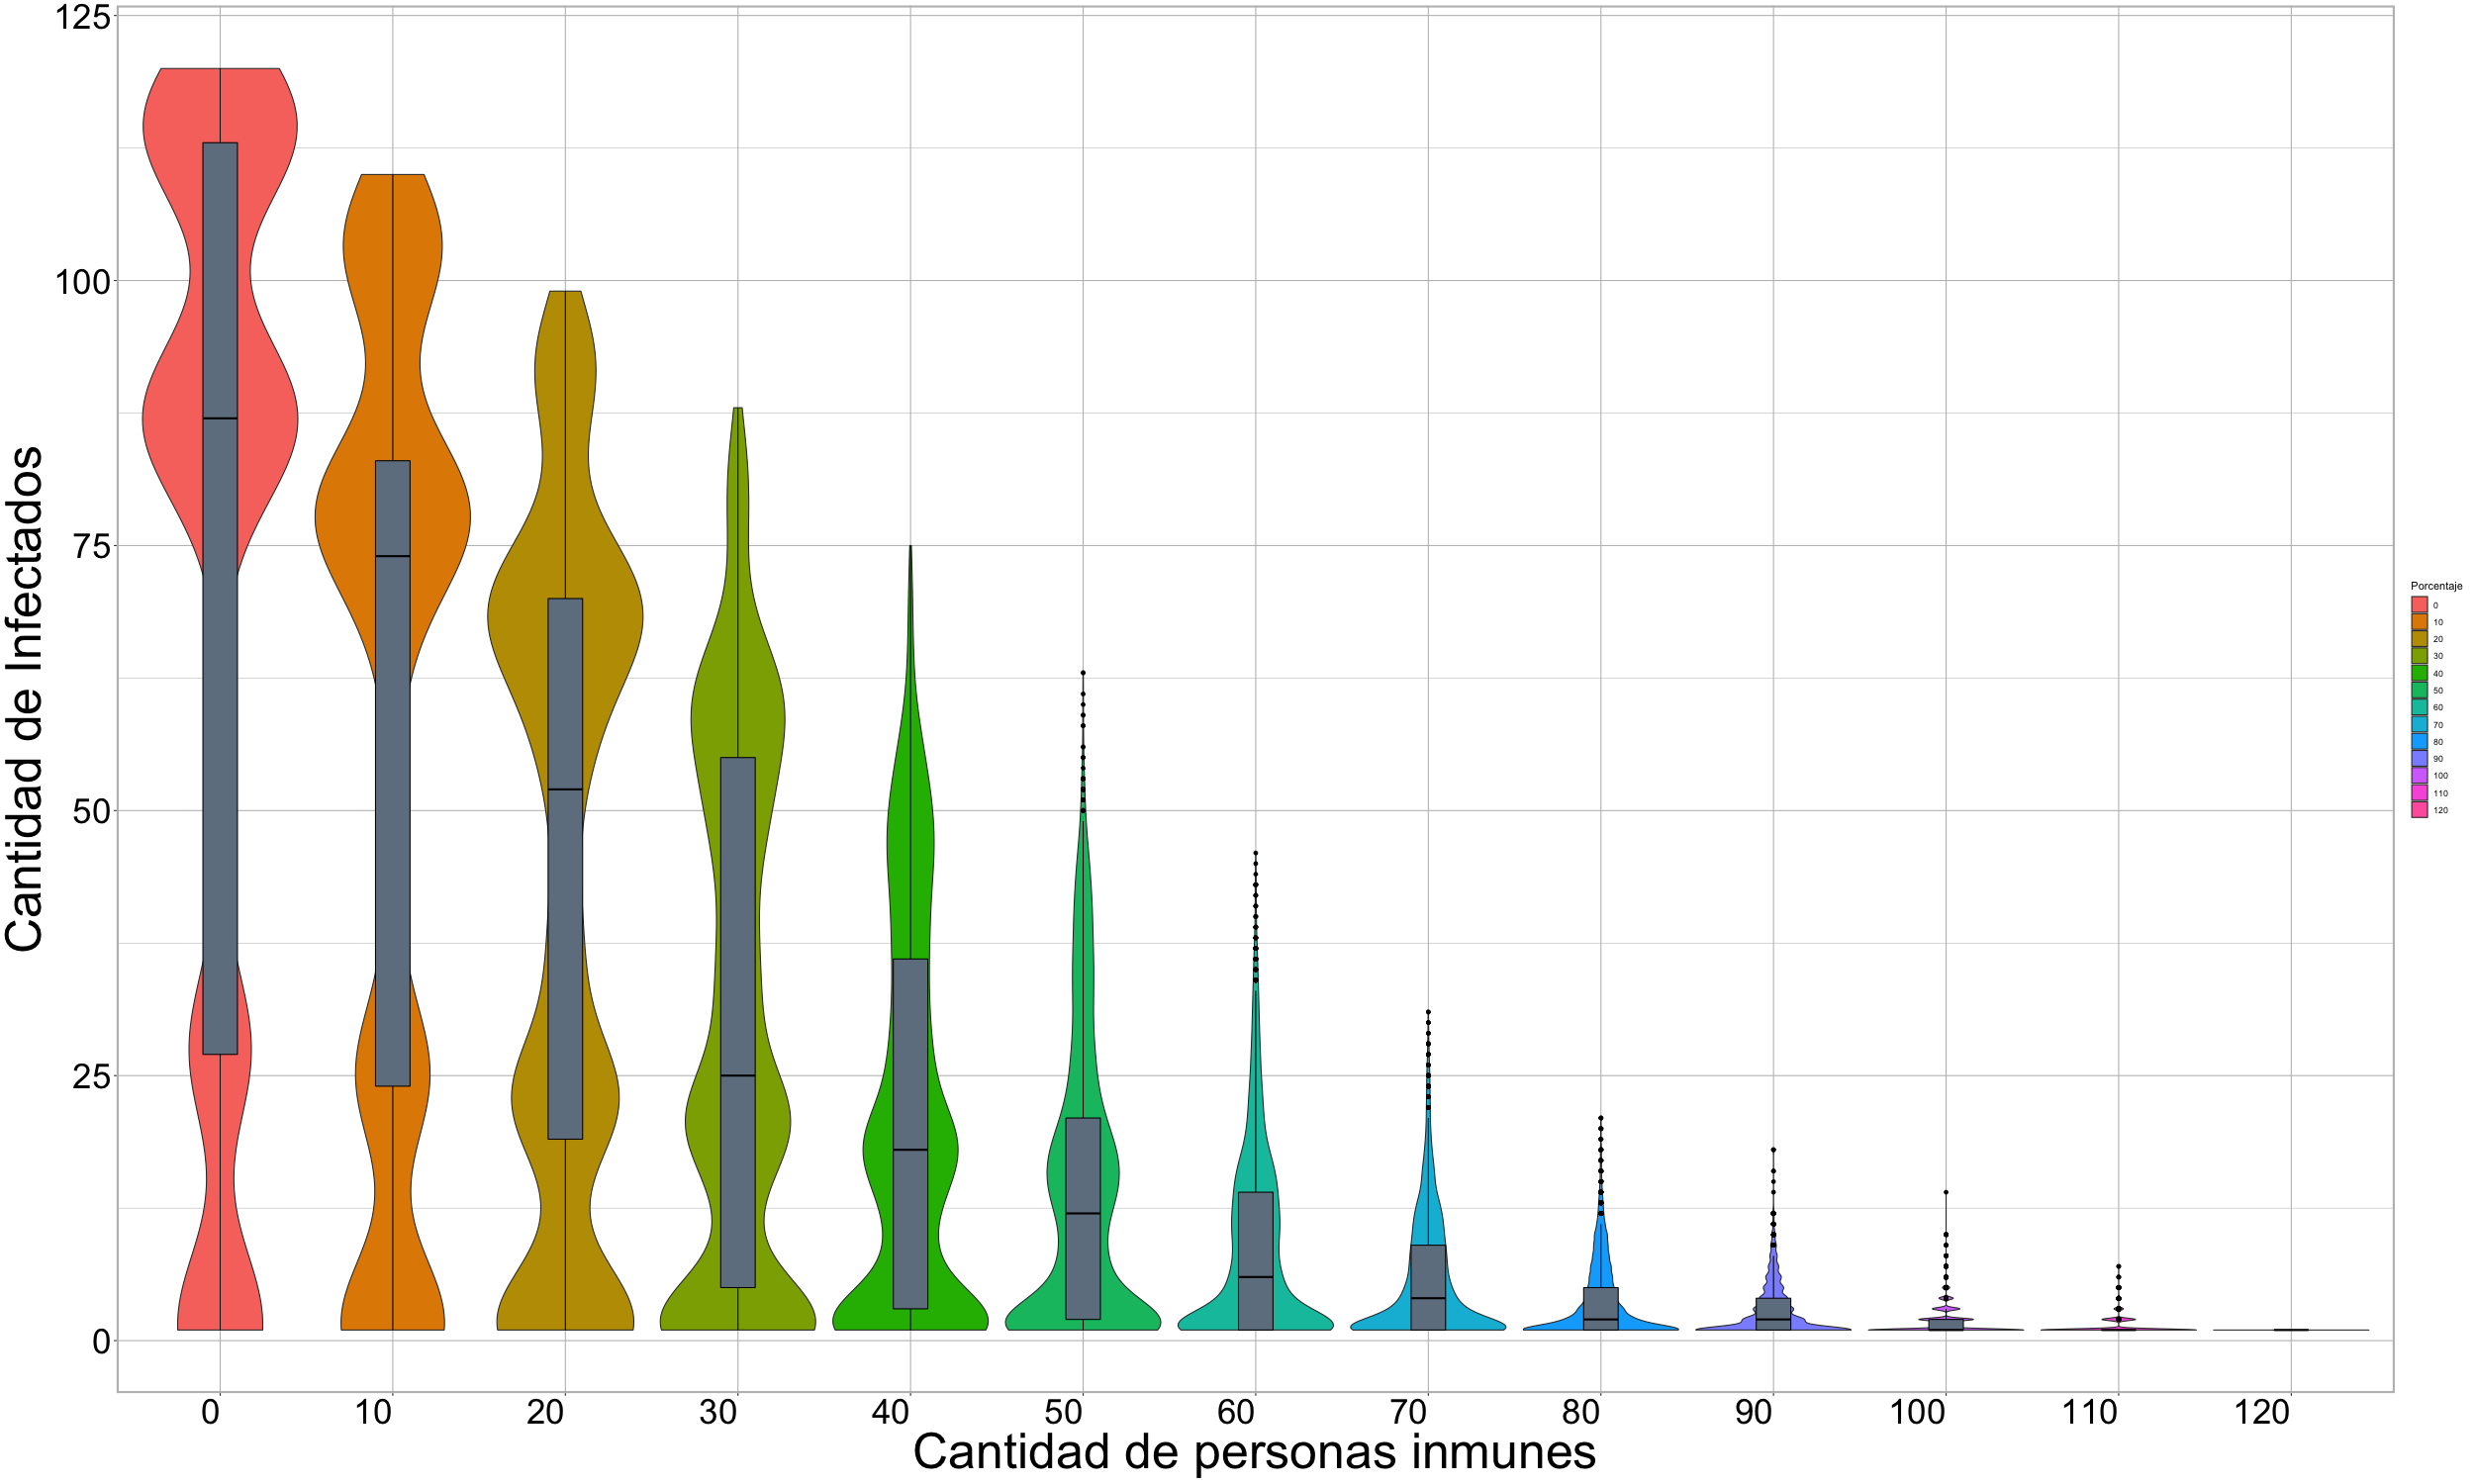
\includegraphics[scale=0.18]{Tesis/img/random.png}
    \caption{Vacunando nodos al azar de la red.}
    \label{fig:random}
\end{figure}

\section{Cubrebocas}



\begin{figure}
    \centering
    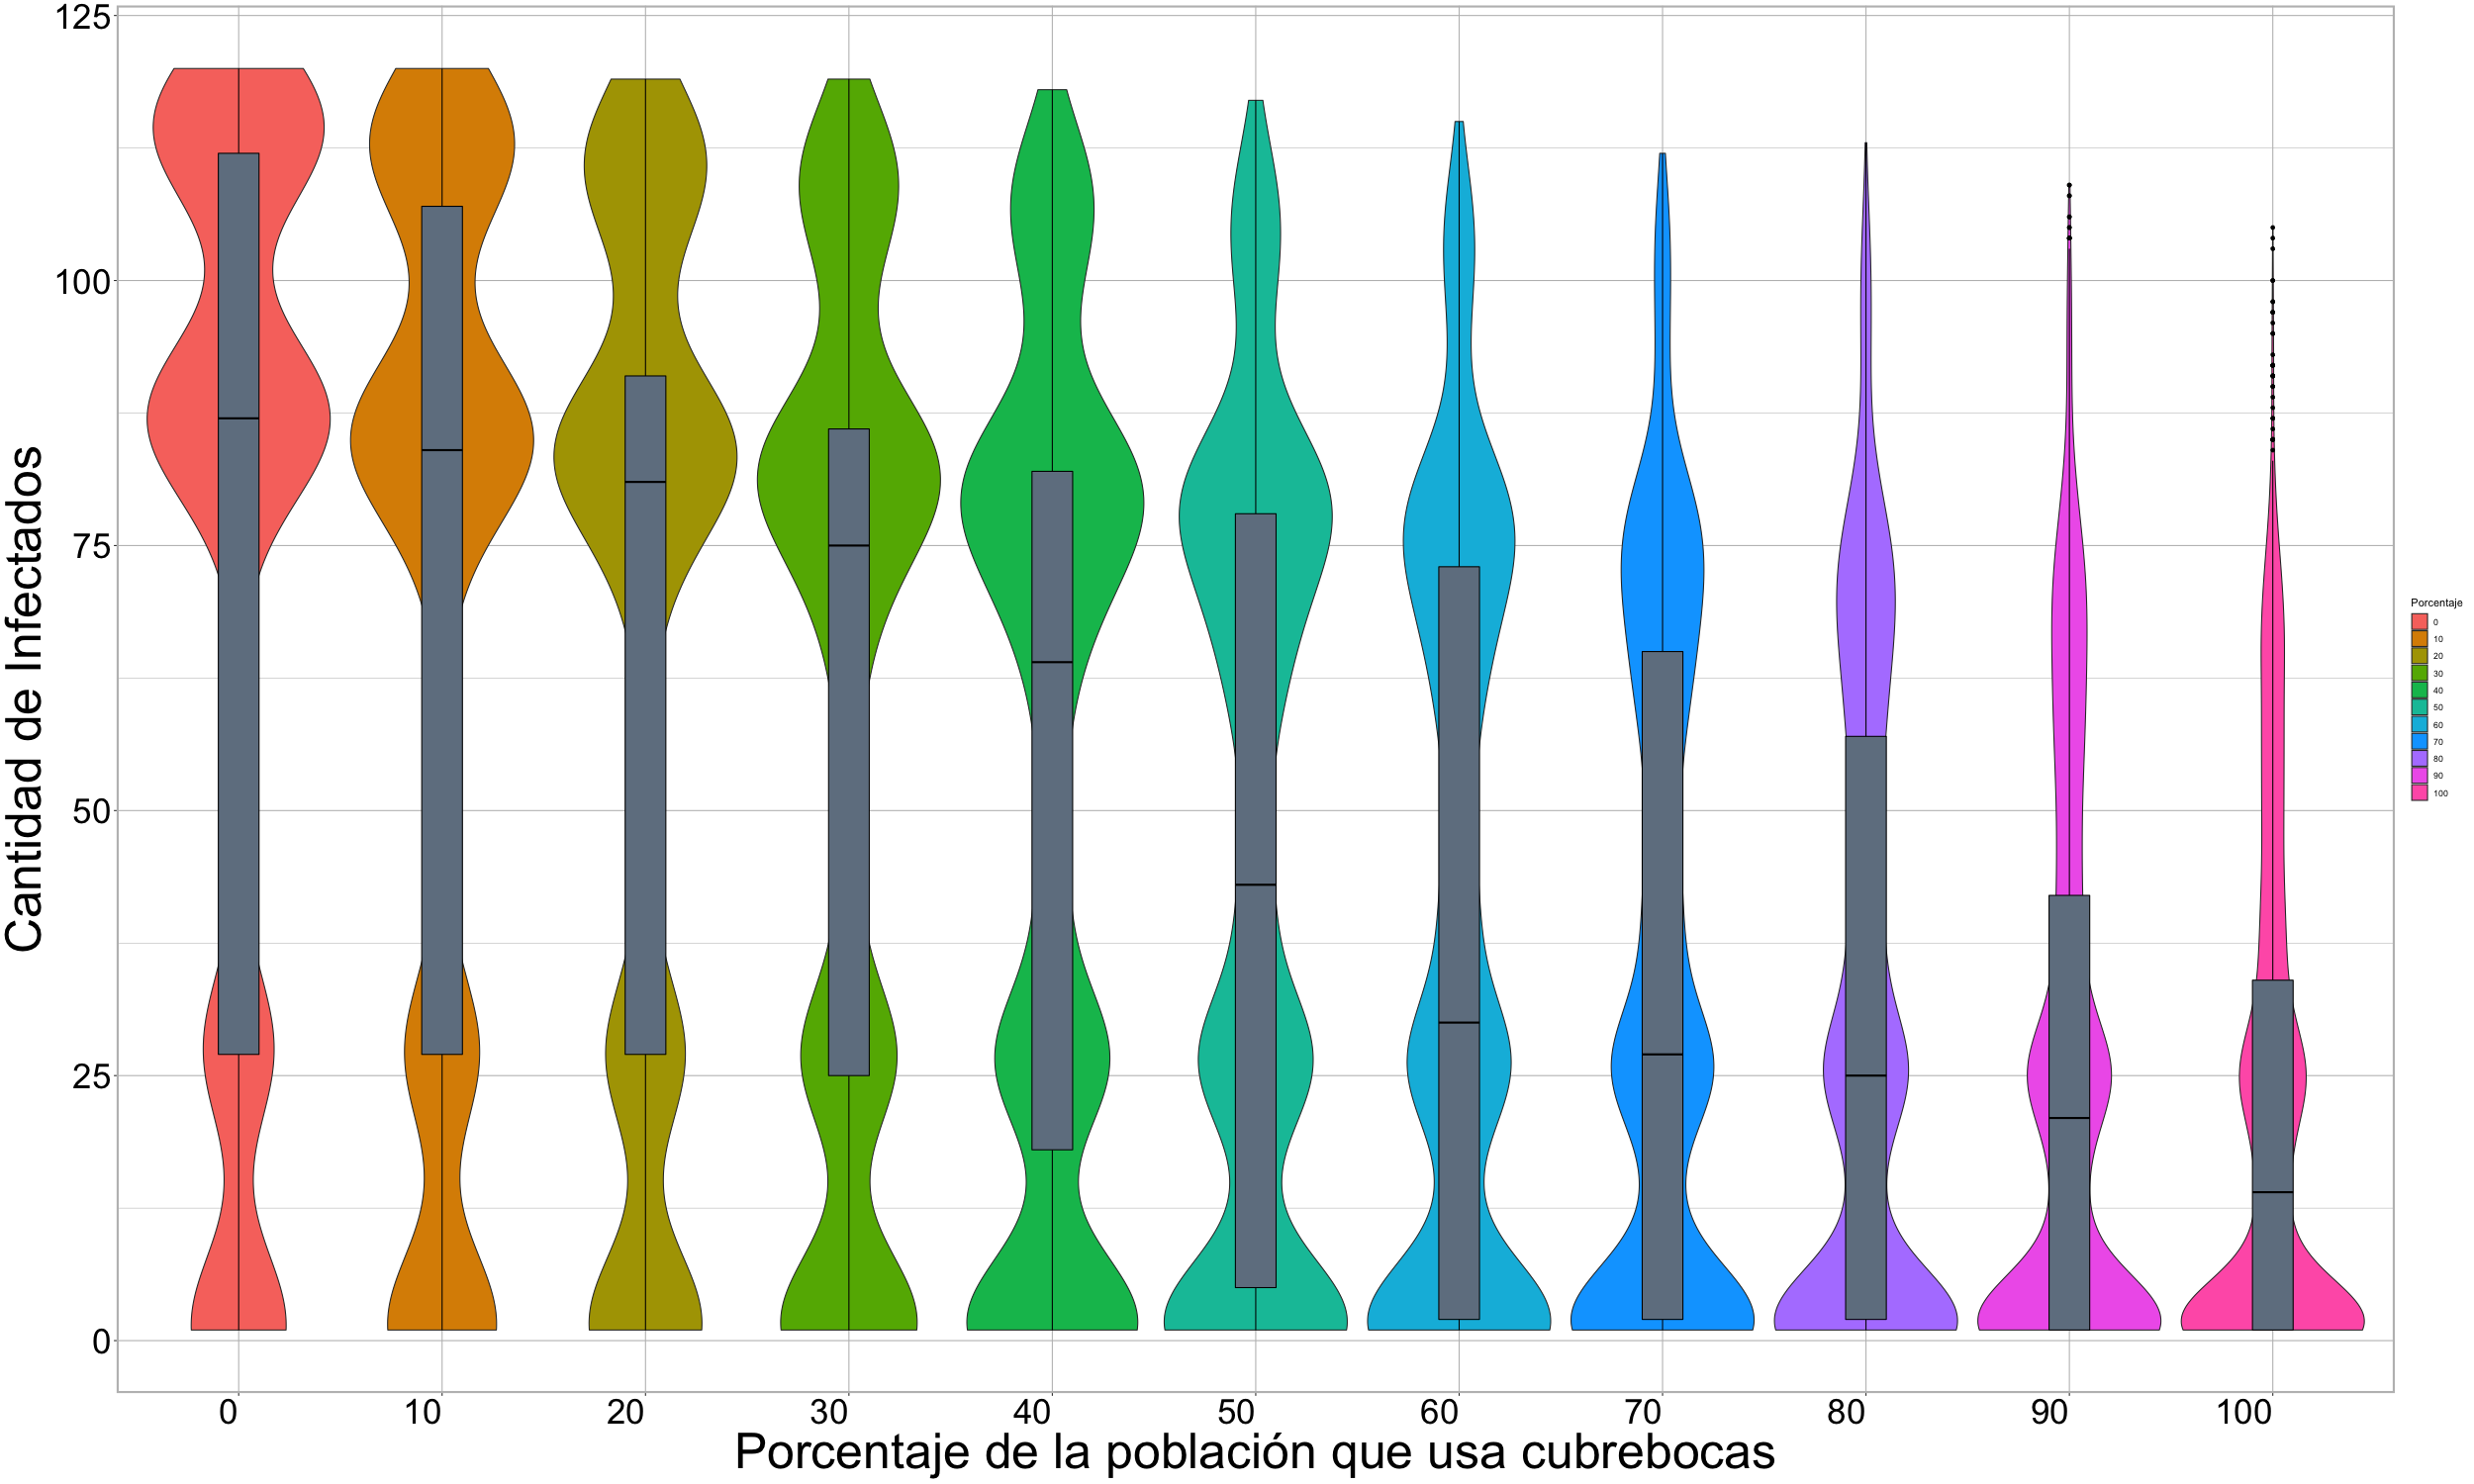
\includegraphics[scale=0.18]{Tesis/img/face-mask.png}
    \caption{Cubrebocas.}
    \label{fig:face-mask}
\end{figure}

\section{Aislamiento}

\begin{figure}
    \centering
    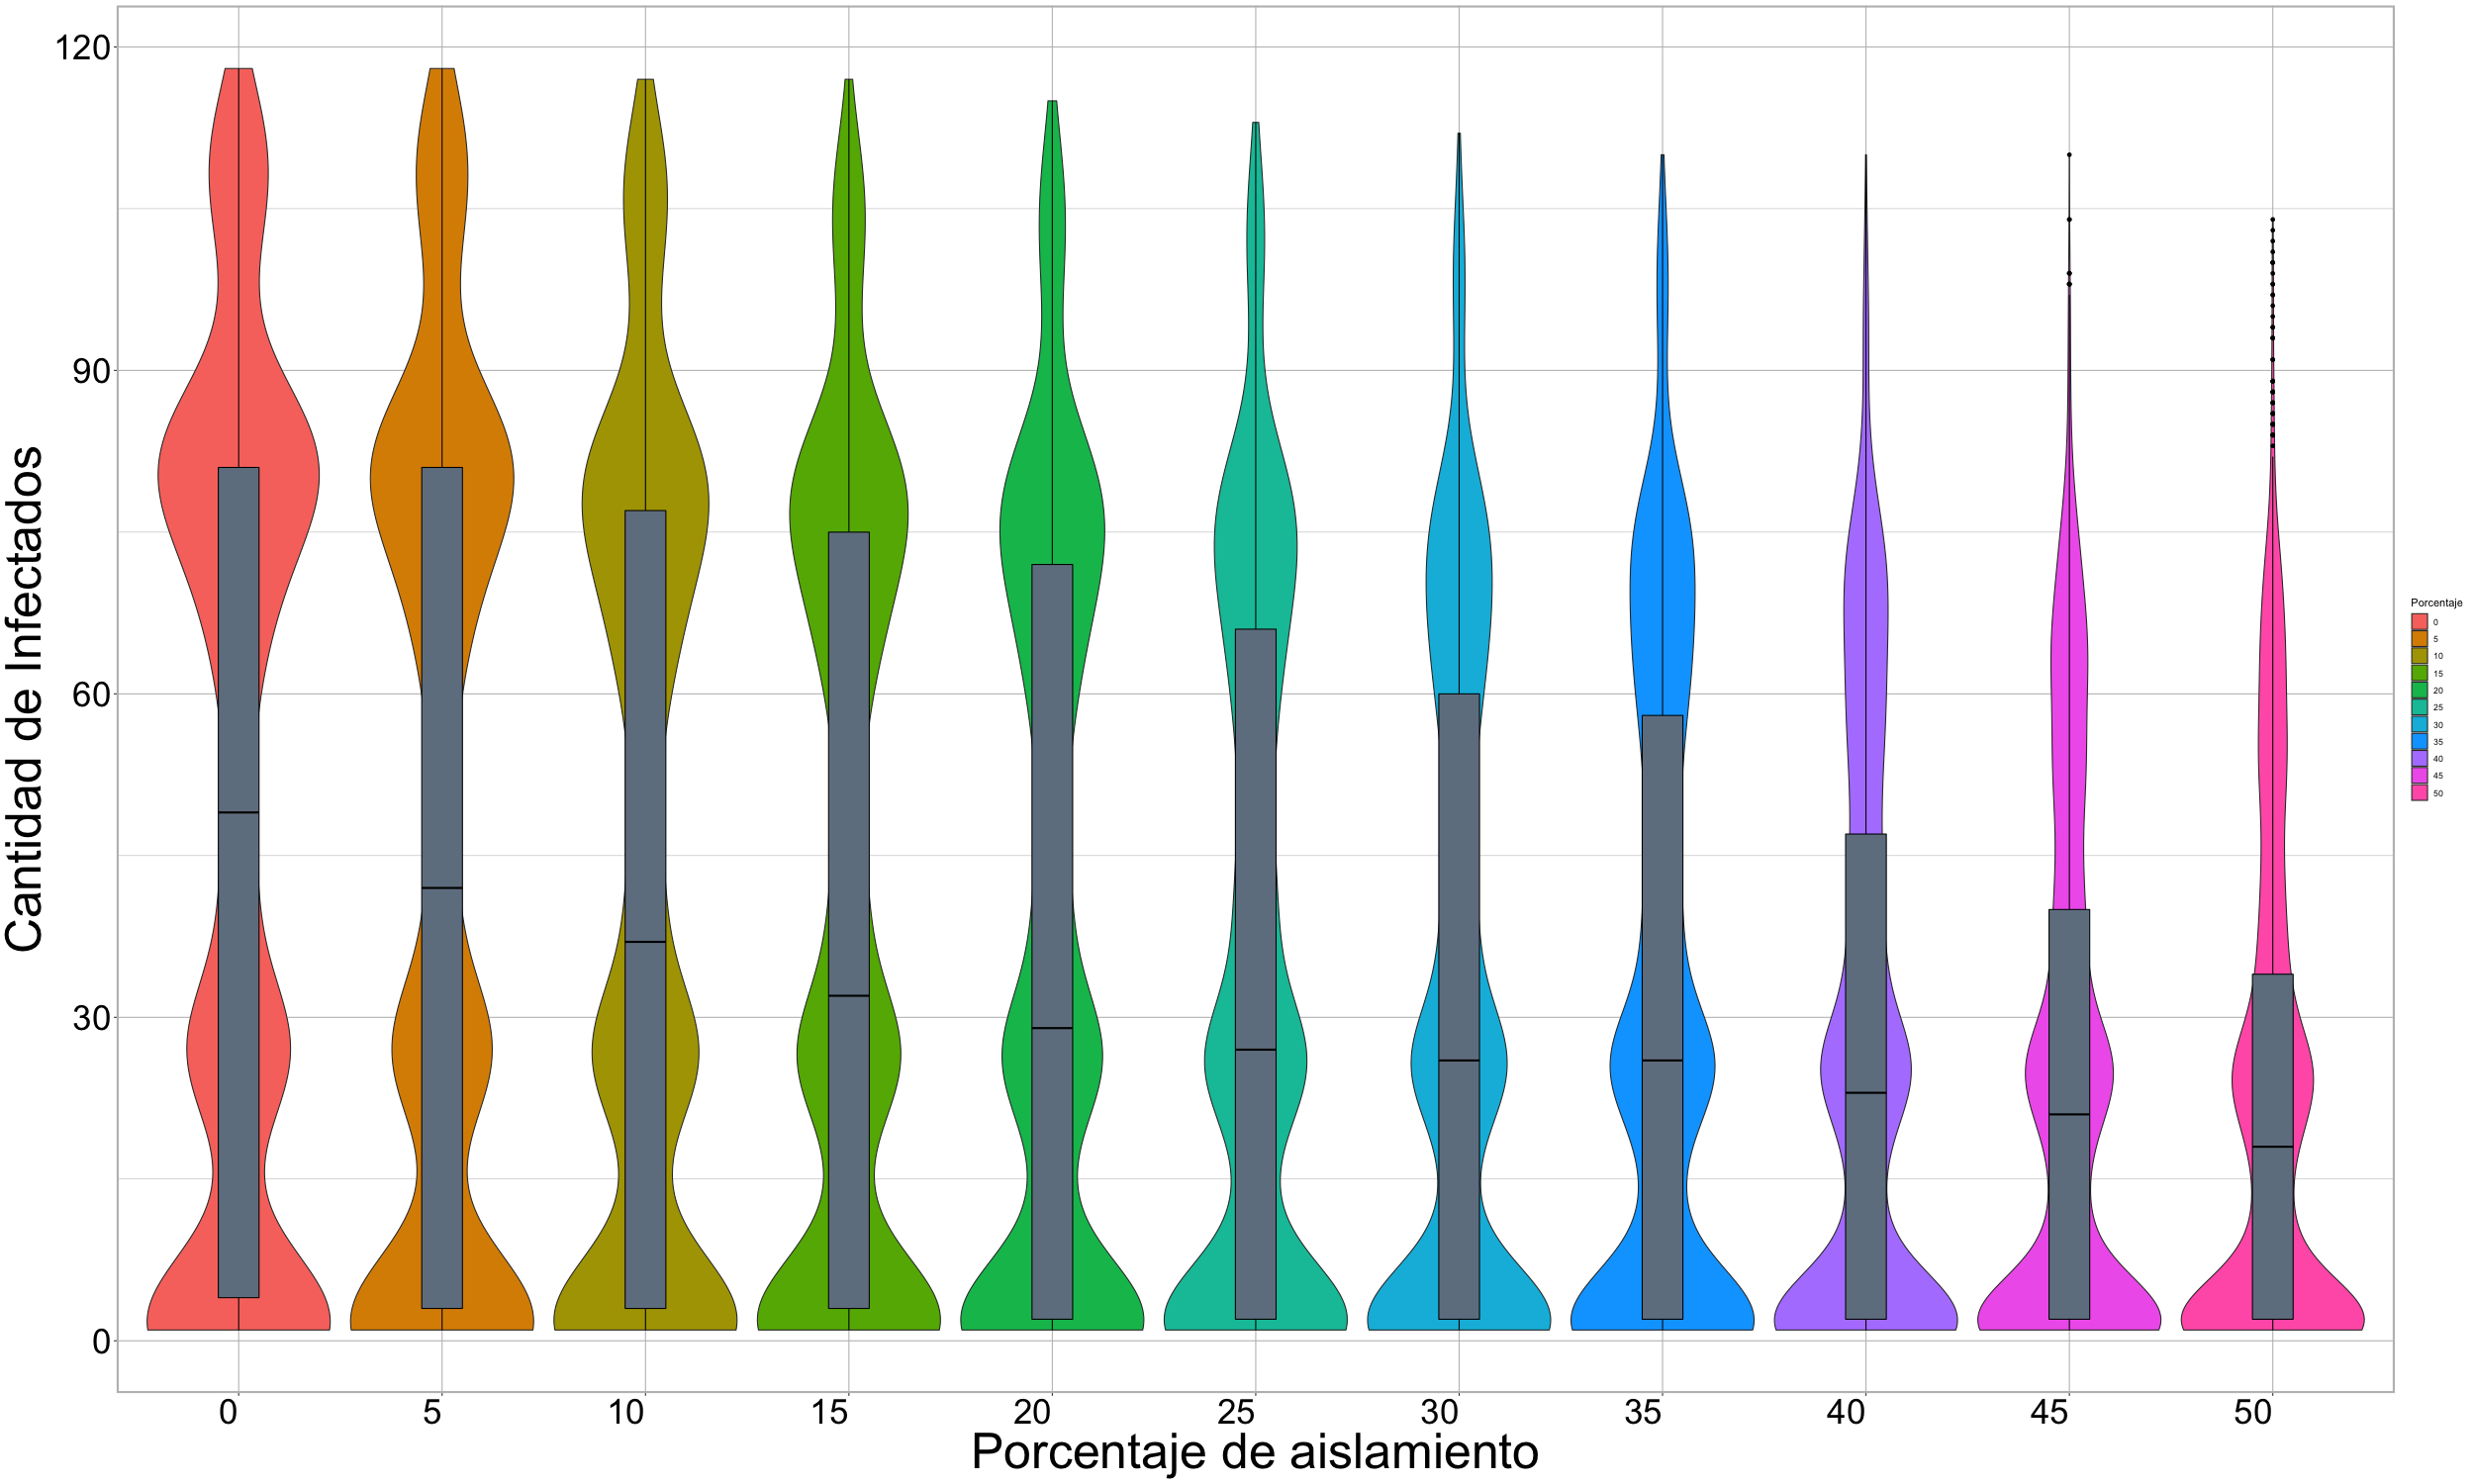
\includegraphics[scale=0.18]{Tesis/img/isolation.png}
    \caption{Aislamiento.}
    \label{fig:isolation}
\end{figure}